\section{Mathematical Flexibility}

\lstset{
	basicstyle=\footnotesize
}


\subsection{Design}
\begin{frame}{Mathematical Flexibility: Motivation}
	\begin{itemize}
		\item Mathematical system is the language of specification
		\item It is the source of an increase in effort for verified software
		\item Therefore, it needs to be familiar and its results reusable
		\item Pure systems contain many useful features that practical systems do not take advantage of
	\end{itemize}
\end{frame}

\begin{frame}{Mathematical Flexibility: Contributions}
	\begin{itemize}
		\item We demonstrate how a number of features from pure systems (higher-order definitions, first-class types, etc.) can be utilized to ease the verification task in a practical system
		\item We provide a mathematical foundation for several pre-existing RESOLVE features
		\item We introduce novel tools for static reasoning in the presence of dependent types
		\item For full details, see Chapter 5
	\end{itemize}
\end{frame}



\begin{frame}{Tools for Static Reasoning}
	\begin{itemize}
		\item First-class types permit undecidable type relationships
		\item Nonetheless, static typing is a useful tool
		\item \emph{Type theorems} are a novel compromise introduced by this research
	\end{itemize}
	\vspace{2em}
	\lstinputlisting[language=resolve,caption=]{examples/typeTheorem1.mt}
\end{frame}

\begin{frame}{Tools for Static Reasoning}
	\begin{figure}
		\centering
		\includegraphics[width=.6\textwidth]{../typeGraph.png}
	\end{figure}
\end{frame}


\subsection{Evaluation}
\begin{frame}{Sorting a Queue}
	\lstinputlisting[basicstyle=\tiny,language=resolve,caption=]{../mathEval/examples/Sorting_Capability.en}
\end{frame}

\begin{frame}{Sorting a Queue}
	\lstinputlisting[basicstyle=\tiny,language=resolve,caption=]{../mathEval/examples/String_Theory1.mt}
\end{frame}

\begin{frame}{Sorting a Queue}
	\lstinputlisting[basicstyle=\tiny,language=resolve,caption=]{examples/String_Theory2.mt}
\end{frame}

\begin{frame}{Sorting a Queue}
	\lstinputlisting[basicstyle=\tiny,language=resolve,caption=]{../mathEval/examples/totalpreorderingvc.asrt}
\end{frame}

\begin{frame}{Sorting a Queue}
	\lstinputlisting[basicstyle=\scriptsize,language=resolve,caption=]{examples/preorderingTheorem.mt}
\end{frame}

\begin{frame}{Error Analysis and Reporting}
~
\end{frame}


\begin{frame}{Array Realization of a Stack}
	\lstinputlisting[basicstyle=\tiny,language=resolve,caption=]{../mathEval/examples/Array_Realiz1.rb}
\end{frame}

\begin{frame}{Array Realization of a Stack}
	\lstinputlisting[basicstyle=\tiny,language=resolve,caption=]{../mathEval/examples/Binary_Iterator_Theory1.mt}
\end{frame}

\begin{frame}{Error Analysis and Reporting}
~
\end{frame}


\begin{frame}{Classroom Experiment}
	\begin{itemize}
		\item Mathematical development assignment given to a graduate-level programming languages class for extra-credit
		\item Example demonstrating first-class types and type theorems
		\item No formal training
		\item Assignment asked increasingly difficult questions: last three required analysis and adaptation\\
		\begin{enumerate}
			\item Asserts that \texttt{Without\_Last\_Zero(10)~=~1}.  This may require an extra step to establish proper symbols.
			\item Asserts that for any multiple of ten, \texttt{t,~Next\_Even(t)~mod~10~=~2}.  This may require some additional steps to establish proper symbols and relationships.
			\item Asserts that for all multiples of ten, \texttt{t}, and integers, \texttt{i}, \texttt{Without\_Last\_Zero(t~*~i)~=~i}.  This may require some additional steps.
		\end{enumerate}
	\end{itemize}
\end{frame}

\begin{frame}{Classroom Experiment}
	\begin{itemize}
		\item 7/9 students participated
		\item All but one student successfully completed questions 10 and 11 correctly
		\item Two of the seven completed 12 correctly
	\end{itemize}
\end{frame}


